%-----------------------------------------------------
In diesem Abschnitt werden die technischen Grundlagen für diese Arbeit vorgestellt und das Wichtigste erörtert. Es kann nicht im vollem Umfang auf die Details der Technik eingegangen werden ohne den Rahmen dieser Arbeit zu sprengen. Interessierte sei die referenzierte Literatur für eine weite Lektüre empfohlen.
%
\subsection{RFID}
%
Bei \textit{Radio-Frequency Identification} (RFID) handelt es sich um einen Funkstandard der die kontaktlose Identifikation bei gleichzeitiger Erfassung zusätzlicher Informationen ermöglicht. Zur Technik gehört ein Auslesegerät (Reader) und ein oder mehrere Transponder (Tags). Eine sehr grobe Übersicht über typische Bauformen von Tags und Reader ist in \ref{fig:RFID_TAGS_AND_READER} zu finden.  Heute verfügbare Transponder lasen sich auf nahezu jeder beliebigen Oberfläche anbringen lassen. Das ermöglicht ein großes Anwendungsspekrum, praktisch wird die Technik in jeder Umgebung eingesetzt in der es erforderlich oder nützlich ist, Dinge kontaktlos zu identifizieren. Eine gute Übersicht über Branchen und Anwendungsgebiete für RFID ist in \cite{RFIDJournal} zu finden. Im Rahmen dieser Arbeit wird kein umfassender Überblick über die Technik geboten, da die Bauformen und Spezifikationen sehr stark variieren. Eine gute Einführung und Übersicht zur Technik ist in \cite{finkenzeller2008rfid} zu finden. Dort werden auch detailliert die physikalischen Grundlagen von erläutert. Aufgrund des großen Anwendungsspektrums und der weiten Verbreitung ist die Technik in die Kritik geraten. Unter dem Dach des Vereins digitalcourage e.V. exisitiert die Kampange \textit{StopRFID}. Die Kampagne hat sich zum Thema gemacht über die Anwendungsmöglichkeiten und Gefahren von RFID aufzuklären \cite{stoprfid2013}. Die Seiten der Kampagne bieten eine sehr weitgehende Auflistung der Anwendungen für RFID. Ziel der Kampagne ist es die Gefahren in den gesellschaftlichen Fokus zu rücken und für den Umgang mit der allgegenwärtigen Technik zu sensibilisieren. Die Kampagne über sich selbst:
\begin{quote}
"Wir wollen RFID nicht komplett verhindern. Es geht uns nicht darum, die RFID-Entwicklung zum Erliegen zu bringen ... Im Gegenteil." \footnote{\url{http://www.foebud.org/rfid/was-kann-ich-tun/}}
\end{quote}
%
\begin{figure} [h]
\centering
         \caption[Beispiele für Transponder und Lesegeräte]{ Hier gezeigt sind Beispiele für Transponder und Lesegeräte. Das linke Bild zeigt drei typische Tags, nahezu jede Gestalt ist mittlerweile erhältlich. Die hier gezeigten Tags eignen sich für eine Anbringung an glatten Oberflächen. Es gibt zig weitere Bauformen, die unterschiedlichste Anwendungsspektren bedienen und sogar eine Implantation ermöglichen (nicht gezeigt). Im rechten Bild ist ein Handlesegerät gezeigt. Zum Mobilen Auslesen über mittlere bis kurze Distanzen. Auch bei den Readern gibt es unterschiedlichste Bauformen, die je nach Anwendungsfall ausgewählt werden. }
         \label{fig:RFID_TAGS_AND_READER}
         \vspace{0.5cm}%         
         \begin{subfigure}[h]{0.4\textwidth}
                 \centering
                 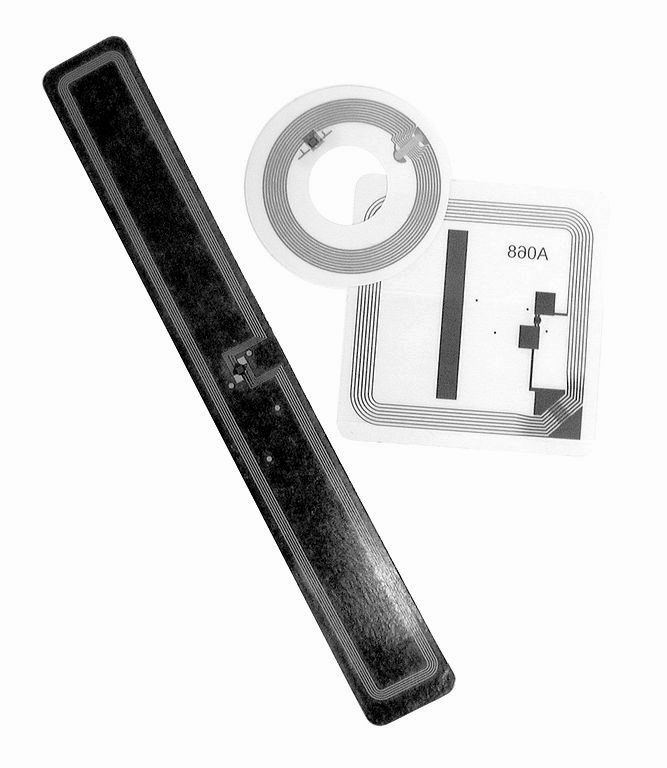
\includegraphics[width=\textwidth]{img/667px-RFID_Tags_gs.png}
                 \vspace{.1cm}
                 \caption{ RFID- Transponder }
                 \label{fig:TAGS}\textit{}
         \end{subfigure}
%         
\qquad
%
         \begin{subfigure}[h]{0.4\textwidth}
                 \centering
                 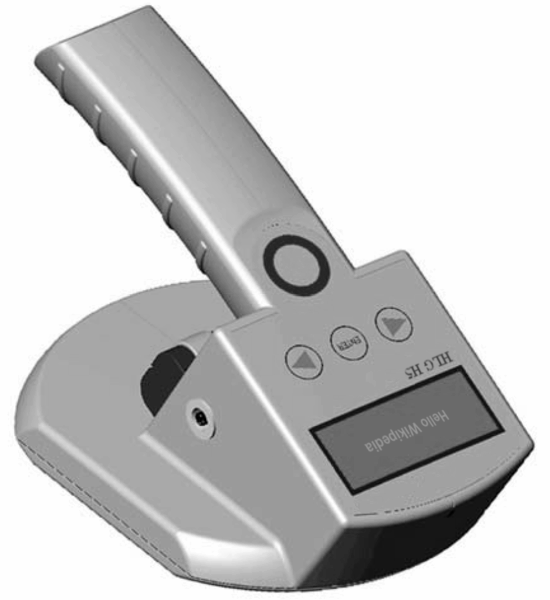
\includegraphics[width=\textwidth]{img/RFID-Reader_gs.png}
                 \vspace{.1cm}
                 \caption{ RFID- Handlesegerät }
                 \label{fig:READER}
         \end{subfigure}
\end{figure}
%
\label{sec:Measurement1}
%
\begin{enumerate}
	\item Die Messung der Position erfolgt über die Auswertung der Phasenlage des empfangenen Signals in Bezug auf ein Referenzsignal. In der EU gibt es verschiedene, zulässige RFID-Frequenzen\footnote{insert reference here} (865,5?867,5 MHz) kann man die Wellenlänge mit: $ \lambda\simeq0,35 m $ angeben. Daraus folgt, dass alle 35 cm die gleiche Konfiguration der Phase vorliegt. Im Rahmen dieser Arbeit wird dabei von \textit{Isophasen} gesprochen. Die gewonnene Information aus der Phase ist nicht eindeutig, d.h. es lässt sich durch die Kenntnis der Phase nicht unmittelbar auf die korrekte Postion schließen. Man kann das Problem umgehen in dem man auf die errechnete Position ein ganzzahliges Vielfaches der Wellenlänge addiert. Die sog. Wellenzahl (siehe~\eqref{eq:Wavenumbers}).
	\item Das System der Amedo STS verwendet eine spezielle Antennenanordnung um die Position zu ermitteln. Dabei wird eine Antennenanzahl >4 eingesetzt. Für jede dieser Antennen muss eine eigene Wellenzahl bestimmt werden. Durch Auslöschung des Signals, Absorption etc. kann es dazu kommen, dass eine Antenne eine unbestimmte Zeit lang kein Signal vom Tag empfängt. Wenn die Antenne nach dieser Zeit erneut ein Signal empfängt ist die ihr zugehörige Wellenzahl unbekannt und muss neu bestimmt werden. 
	\item In realen Umgebungen treten zusätzlich noch Ruflektionen und ein sog. Multipath-Effekt auf. Dabei wird das Signal nicht auf dem Direkten Weg Antenne-Tag-Antenne empfangen sondern über einen unbekannten, längeren Weg. Dadurch kommt es zu einem Fehler in der Phase. Zusätzlich ist dieser Effekt individuell für jede Antenne.
\end{enumerate}
%
\begin{figure}[h]
         \centering
         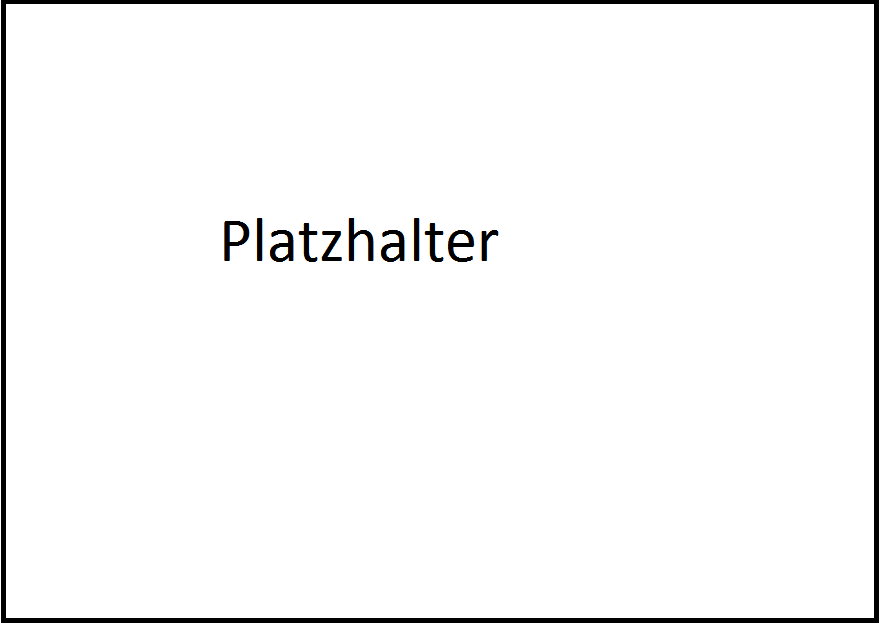
\includegraphics[width=0.5\textwidth]{img/00_placeholder.png}
         \caption[Messystem der Amedo GmbH]{Das Bild zeigt das PRPS-Messystem zu erkennen sind die wesentlichen elektronischen Komponenten, sowie weitere periphere Hardware }
         \label{fig:System}
\end{figure}
%
\begin{figure}[h]
         \centering
         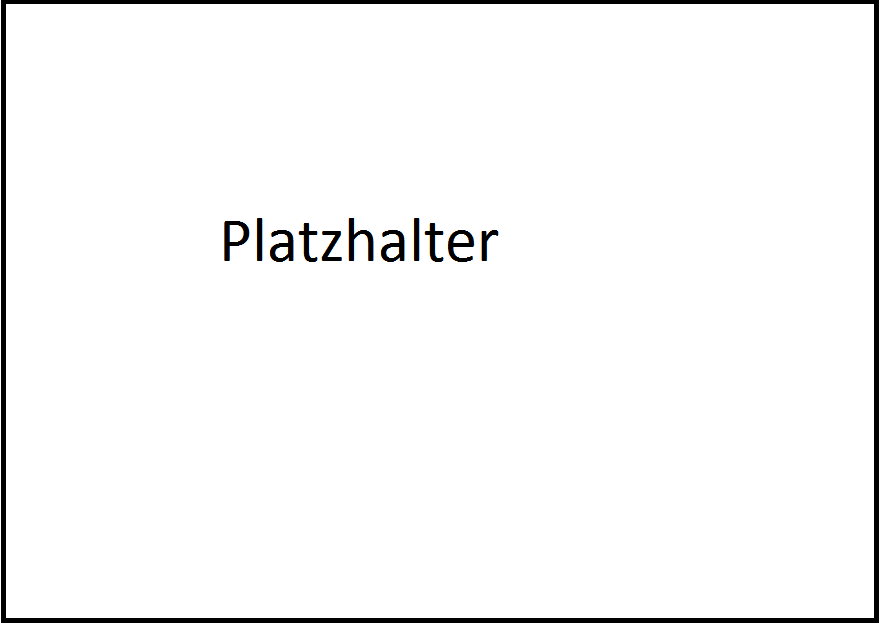
\includegraphics[width=0.5\textwidth]{img/00_placeholder.png}
         \caption[Messaufbau der Amedo GmbH]{Abgebildet ist der Messaufbau mit unterschiedlichen Antennen}
         \label{fig:Setup}
\end{figure}
\subsection{Messystem der Amedo GmbH}
%
\lipsum[1-2]
%